\documentclass{article}
\input{Headers/header}
\input{Headers/formal}

\fancyhead[L]{Теория вероятности}

\let\eps\varepsilon

\newcommand{\A}{{\mathfrak A}}
\newcommand{\B}{{\mathfrak B}}

\begin{document}
    \tableofcontents
    \section{Основы теории вероятности.}
    \paragraph{Вероятностное пространство.}
    \begin{definition}
        Пусть $\Omega$~--- множество, тогда $\A\in 2^\Omega$ называется \textbf{алгеброй}, если
        \begin{enumerate}
            \item $\Omega\in A$.
            \item $\forall A\in\mathfrak A~\overline A\in\A$. Здесь и далее $\overline A=\Omega\setminus A$.
            \item $\forall A,B\in\A~A\cup B\in\A$.
        \end{enumerate}
        При этом $\Omega$ называется \textbf{множеством элементов событий}, $\A$~--- \textbf{набор событий}, $A\in\A$~--- \textbf{событие}, $A\cup B=A+B$~--- \textbf{сумма событий}, $\overline A$~--- \textbf{противоположное событие}, $A\cap B=AB$~--- \textbf{произведение событий}.
    \end{definition}
    \begin{definition}
        Алгебра является \textbf{сигма-алгеброй}, если она замкнута относительно объединения счётного количества своих элементов.
    \end{definition}
    \begin{definition}
        Пусть $\A$~--- сигма-алгебра на $\Omega$. Пусть $P\colon \A\to\mathbb [0;+\infty)$ и
        \begin{enumerate}
            \item $P(\Omega)=1$.
            \item Если $\{A_i\}_{i=1}^\infty\subset\A$ и $\forall A_iA_j=\varnothing$ то
            $$
            P\left(\bigcup\limits_{i=1}^\infty A_i\right)=\sum\limits_{i=1}^\infty P(A_i)
            $$
        \end{enumerate}
        Тогда $(\Omega;\A;P)$ называется \textbf{вероятностным пространством}.
    \end{definition}
    \begin{definition}
        Пара событий называется \textbf{несовместной}, если их пересечение пусто. Набор событий \textbf{несовместен}, если они попарно несовместны.
    \end{definition}
    \begin{definition}
        Пусть $A\subset2^\Omega$~--- алгебра. Тогда минимальная по включению сигма-алгебра $\sigma(A)\supset A$ называется \textbf{минимальной сигма-алгеброй}.
    \end{definition}
    \begin{claim}
        Таковая существует.
    \end{claim}
    \begin{proof}
        Хотя бы одна такая существует ($2^\Omega$), причём если пересечь сколько угодно сигма-алгебр, то получится искомая сигма-алгебра.
    \end{proof}
    \begin{definition}
        Пусть $\A$~--- алгебра на $\Omega$, $P\colon\A\to[0;+\infty)$ и
        \begin{itemize}
            \item $P(\Omega)=1$.
            \item Если $\{A_i\}_{i=1}^\infty\subset\A$ и $\bigsqcup\limits_{i=1}^\infty A_i\in\A$, то
            $$
            P\left(\bigsqcup\limits_{i=1}^\infty A_i\right)=\sum\limits_{i=1}^\infty P(A_i)
            $$
        \end{itemize}
        Тогда $(\Omega;\A;P)$~--- \textbf{вероятностное пространство в широком смысле}.
    \end{definition}
    \begin{theorem}[О продолжении меры]
        Пусть $(\Omega;\A;P)$~--- вероятностное пространство в широком смысле. Тогда существует единственная функция вероятности $Q\colon\sigma(\A)\to[0:+\infty)$, такое что $Q\Big|_{\A}\equiv P$.\\
        Без доказательства.
    \end{theorem}
    \begin{remark}
        Эта теорема позволяет нам сказать, например, что мы хотим задать вероятность на отрезках.
    \end{remark}
    \begin{definition}
        \textbf{Борелевская сигма-алгебра}~--- минимальная $\sigma$-алгебра, которая содержит все открытые множества.
    \end{definition}
    \begin{example}
        Дискретное вероятностное пространство: $\Omega=\{\omega_i\}_{i=1}^N$, $A=2^\Omega$, $P(\{\omega_i\})=p_i$, $\sum p_i=1$. Тогда $P(A)$~--- сумма вероятностей элементов $A$.
    \end{example}
    \begin{example}
        Геометрическая вероятность: $\Omega\subset\mathbb R^n$, измеримо по Лебегу, $\mu A<+\infty$, $\A$ состоит из измеримых по Лебегу множеств, $P(A)=\frac{\mu A}{\mu\Omega}$. Обычно при этом $\mathbb R^n$ не более чем трёхмерно.
    \end{example}
    \paragraph{Свойства вероятности.}
    \begin{property}
        $$
        \forall A,B\in\A~A\subset B\Rightarrow P(A)\leqslant P(B)
        $$
    \end{property}
    \begin{proof}
        Понятно, что $B\setminus A\in\A$. Тогда
        $$
        B=A\sqcup(B\setminus A)\Rightarrow P(B)=P(A)+P(B\setminus A)\geqslant P(A)
        $$
    \end{proof}
    \begin{corollary}
        $$\forall A\in\A~P(A)\leqslant1$$
    \end{corollary}
    \begin{property}
        $$
        P(A)=1-P(\overline A)
        $$
    \end{property}
    \begin{property}
        $$
        P(A+B)=P(A)+P(B)-P(AB)
        $$
    \end{property}
    \begin{proof}
        $$
        B=(B\setminus AB)\sqcup AB\Rightarrow P(B)=P(B\setminus AB)+P(AB)
        $$
        Тогда
        $$
        P(A+B)=P(A)+P(B\setminus AB)=P(A)+P(B)-P(AB)
        $$
    \end{proof}
    \begin{claim}[Формула включений-исключений]
        $$
        P(A_1+\cdots+A_n)=\sum\limits_{i=1}^nP(A_i)-\sum\limits_{\substack{i,j=1\\i<j}}^nP(A_iA_j)+\sum\limits_{\substack{i,j,k=1\\i<j<k}}^nP(A_iA_jA_k)-\cdots+(-1)^nP(A_1\cdots A_n)
        $$
    \end{claim}
    \begin{proof}
        Мне лень это писать, докажите сами по индукции.
    \end{proof}
    \begin{claim}
        $$
        P\left(\bigcup\limits_iA_i\right)\leqslant\sum\limits_i P(A_i)
        $$
    \end{claim}
    \begin{proof}
        Пусть $B_1=A_1$, $B_2=A_2\overline{A_1}$, $B_3=A_3\overline{A_1\cup A_2}$ и так далее. Тогда
        $$
        \bigcup\limits_iA_i=\bigsqcup\limits_iB_i
        $$
        При этом $B_i\subset A_i$, а значит
        $$
        \sum\limits_i P(A_i)\geqslant\sum\limits_i P(B_i)
        $$
    \end{proof}
    \begin{theorem}
        Пусть $(\Omega;\A;P)$~--- вероятностное пространство. Тогда следующие утверждения равносильны:
        \begin{enumerate}
            \item $P$ счётно-аддитивна.
            \item $P$ конечно-аддитивна и $\forall \{B_i\}_{i=1}^\infty:B_{i+1}\subset B_i$, $B=\bigcap\limits_{i=1}^\infty B_i$ $\lim\limits_{n\to\infty}P(B_i)=P(B)$ (непрерывность сверху).
            \item $P$ конечно-аддитивна и $\forall \{C_i\}_{i=1}^\infty:C_{i+1}\supset B_i$, $C=\bigcup\limits_{i=1}^\infty C_i$ $\lim\limits_{n\to\infty}P(C_i)=P(C)$ (непрерывность сверху).
        \end{enumerate}
    \end{theorem}
    \begin{proof}
        Равносильность двух непрерывностей тривиально из формул де Моргана.\\
        Докажем, что из 1 следует 2. Конечная аддитивность есть, докажем непрерывность сверху. Пусть $A_1=B_1\overline{B_2}$, $A_2=B_2\overline{B_3}$ и так далее. Очевидно, $A_i$ несовместны. Также очевидно, что $A_i$ несовместны с $B$. Также заметим, что
        $$
        B_n=B\sqcup\bigsqcup\limits_{i=n+1}^\infty A_i
        $$
        Отсюда $P(B_n)=P(B)+\sum\limits_{i=n+1}^\infty P(A_i)$, а справа остаток (очевидно, сходящегося) ряда, который стремится к нулю при $n\to\infty$.\\
        Теперь из 2 докажем 1. Рассмотрим $\{A_i\}_{i=1}^\infty$ несовместные. Очевидно,
        $$
        \sum\limits_{i=1}^\infty P(A_i)=\lim\limits_{n\to\infty}\sum\limits_{i=1}^nP(A_i)
        $$
        А ещё мы знаем, что
        $$
        \bigsqcup\limits_{i=1}^\infty A_i=\bigsqcup\limits_{i=1}^nA_i\sqcup\bigsqcup\limits_{i=n+1}^\infty A_i
        $$
        То есть
        $$
        \lim\limits_{n\to\infty}P\left(\bigsqcup\limits_{i=1}^nA_i\right)=
        \lim\limits_{n\to\infty}\left(P\left(\bigsqcup\limits_{i=1}^\infty A_i\right)-P\left(\bigsqcup\limits_{i=n+1}^\infty A_i\right)\right)=
        P\left(\bigsqcup\limits_{i=1}^\infty A_i\right)-\lim\limits_{n\to\infty}P\left(\bigsqcup\limits_{i=n+1}^\infty A_i\right)
        $$
        Второе слагаемое~--- ноль но непрерывности меры, а отсюда счётная аддитивность.
    \end{proof}
    \paragraph{Условная вероятность.}
    \begin{remark}
        Пусть $|\Omega|=n$, $|A|=k$, $|B|=m$, $|AB|=l$. Если мы знаем, что $B$ произошло, как узнать вероятность того, что произошло $A$? Ну, это
        $$
        \frac lm=\frac{l/n}{m/n}=\frac{P(AB)}{P(B)}
        $$
    \end{remark}
    \begin{definition}
        Пусть $(\Omega;\A;P)$~--- вероятностное пространство, $B\in\A$, $P(B)>0$. Тогда \textbf{условной вероятностью} $A$ при условии $B$ называется
        $$
        P(A|B)=\frac{P(AB)}{P(B)}
        $$
        Также обозначается $P_B(A)$.
    \end{definition}
    \begin{property}
        Несложно проверить, что условная вероятность является вероятностью.
    \end{property}
    \begin{claim}[Произведение вероятностей]
        Несложно по определению проверить
        $$
        P(A_1\cdots A_n)=P(A_1)P(A_2|A_1)P(A_3|A_1A_2)\cdots P(A_n|A_1A_2\cdots A_{n-1})
        $$
    \end{claim}
    \begin{theorem}[Формула полной вероятности]
        Пусть $A\in\A$, $B_i\in\A$ несовместны, $A\subset\bigsqcup\limits_{i=1}^nB_i$ (обычно объединение равно $\Omega$), и $\forall i\in[0:n]~P(B_i)>0$. Тогда
        $$
        P(A)=\sum\limits_{i=1}^nP(A|B_i)P(B_i)
        $$
    \end{theorem}
    \begin{proof}
        $$
        P(A)=P\left(A\cap\bigsqcup\limits_{i=1}^nB_i\right)=P\left(\bigsqcup\limits_{i=1}^nA\cap B_i\right)
        $$
        Всё.
    \end{proof}
    \begin{theorem}[Формула Байеса]
        Пусть $A,B\in\A$, $P(A)>0$, $P(B)>0$. Тогда
        $$
        P(A|B)=\frac{P(B|A)P(A)}{P(B)}
        $$
    \end{theorem}
    \begin{proof}
        Очевидно из определения.
    \end{proof}
    \begin{definition}
        События $A,B\in\A$ называются \textbf{независимыми}, если
        $$
        P(AB)=P(A)P(B)
        $$
    \end{definition}
    \begin{definition}
        Говорят, что $A_1,A_2,\ldots,A_n\in\A$ \textbf{независимы в совокупности}, если
        $P(A_1A_2\cdots A_n)=P(A_1)P(A_2)\cdots P(A_n)$
    \end{definition}
    \begin{property}
        Несложно проверить, что независимость событий $A,B$ равносильна $P(A|B)=P(A)$.
    \end{property}
    \begin{property}
        Независимые в совокупности события попарно независимы. Обратное неверно.
    \end{property}
    \begin{definition}
        Пусть у нас есть два вероятностных пространства: $(\Omega_1,\A_1;P_1)$ и $(\Omega_2,\A_2;P_2)$. Рассмотрим вот такое вероятностное пространство: $(\Omega,\A;P)$, где $\Omega=\Omega_1\times\Omega_2$, $\A$~--- минимальная $\sigma$-алгебра, включающая в себя $\A_1\times\A_2$,
        $$
        P((A_1;A_2))=P_1(A_1)P_2(A_2)
        $$
        Тогда $(\Omega_1,\A_1;P_1)$ и $(\Omega_2,\A_2;P_2)$~--- независимые испытания.
    \end{definition}
    \paragraph{Схема Бернулли.}
    \begin{example}
        Схема Бернулли: $\Omega_1=\{0;1\}$, $\A_1=2^{\Omega_1}$, $P_1(1)=p$, $P_1(0)=1-p=q$. Хочется рассмотреть эту штуку в степени $n$ (то есть $n$ одинаковых независимых испытаний). Тогда что у нас получается для $\omega\in\Omega=\Omega_1^n$?
        $$
        P(\omega)=\sum\limits_{i=1}^nP_i(\omega_i)=p^{\sum\omega_i}q^{n-\sum\omega_i}
        $$
        Посчитаем тут такую вероятность: пусть $S_n$~--- количество успехов в $n$ испытаниях? Посчитаем вероятность того, что $S_n=k$? Очевидно, оно равно $\Cnk nkp^kq^{n-k}$.
    \end{example}
    \begin{claim}
        Пусть $k^*$~--- наиболее вероятное число успехов в Бернуллиевских испытаниях. Тогда
        $$
        k^*=\begin{cases}
            p(n-1)\text{ или }p(n-1)+1 & p(n-1)\in\mathbb N\\
            \lceil p(n-1)-1\rceil & p(n-1)\notin\mathbb N
        \end{cases}
        $$
    \end{claim}
    \begin{proof}
        Давайте рассмотрим вот такое частное:
        $$
        \frac{P(S_n=k+1)}{P(S_n=k)}
        $$
        Чему оно равно?
        $$
        \frac{P(S_n=k+1)}{P(S_n=k)}=\frac{\Cnk n{k+1}p^{k+1}q^{n-k-1}}{\Cnk nkp^kq^{n-k}}=\frac pq\cdot\frac{n-k}{k+1}
        $$
        Нам хочется оценить, больше это чем 1 или меньше (это позволит нам найти $K^*$). Ну,
        $$
        \frac pq\cdot\frac{n-k}{k+1}>1\Leftrightarrow p(n-k)>q(k+1)\Leftrightarrow pn-pk>k=pk+1-p\Leftrightarrow pn>k+1-p\Leftrightarrow pn+p-1>k
        $$
        То есть возрастание достигается при $k<p(n-1)-1$, а иначе убывание. Тогда где экстремум? Рассмотрим $k=p(n-1)-1$. Если это целое число, то там $P(S_n=k+1)=P(S_n=k)$, и это самое $k$ даёт значение больше остальных. То есть $k^*=p(n-1)-1$ или $k^*=p(n-1)$.\\
        А что если оно не целое? То надо куда-то округлить. А именно вверх, потому что тогда оно больше, чем следующее, а предыдущее меньше его.
    \end{proof}
    \begin{example}
        Пусть $n=10000$, $p=\frac1{10000}$. Давайте посчитаем $P(S_n>3)$. Ну, это
        $$
        1-P(S_n\leqslant 3)=1-q^{10000}-10000pq^{10000-1}-\Cnk{10000}2p^2q^{10000-2}-\Cnk{10000}3p^3q^{10000-3}
        $$
        Фиг мы такое посчитаем.
    \end{example}
    \begin{example}
        Или если взять $p=q=0.5$, то при $n=5\cdot10^3$ мы не сможем нормально посчитать $P(S_n=2349)$.
    \end{example}
    \begin{remark}
        Ну и как такое считать?
    \end{remark}
    \begin{theorem}[Теорема Пуассона]
        Пусть у нас есть несколько схем Бернулли. В первой одно испытание и вероятность успеха $p_1$, во второй~--- 2 и вероятность успеха $p_2$, в $n$-ной $n$ испытаний и вероятность $p_n$. Пусть $np_n\underset{n\to\infty}\longrightarrow\lambda>0$. Тогда
        $$
        P(S_n=k)\underset{n\to\infty}\longrightarrow e^{-\lambda}\frac{\lambda^k}{k!}
        $$
    \end{theorem}
    \begin{proof}
        Известно,
        $$
        P(S_n=k)=\frac1{k!}n(n-1)\cdots(n-k+1)p_n^k(1-p_n)^{n-k}
        $$
        Известно, что
        $$
        np_n=\lambda+o(1)\Rightarrow p_n=\frac\lambda n+o\left(\frac1n\right)
        $$
        Тогда
        $$
        P(S_n=k)=\frac1{k!}\cancelto1{n(n-1)\cdots(n-k+1)\frac1{n^k}}\cancelto{\lambda^k}{(\lambda+o(1))^k}\frac{\cancelto{e^{-\lambda}}{\left(1-\frac\lambda n+o\left(\frac1n\right)\right)^n}}{\cancelto1{\left(1-\frac\lambda n+o\left(\frac1n\right)\right)^k}}\underset{n\to\infty}\longrightarrow e^{-\lambda}\frac{\lambda^k}{k!}
        $$
    \end{proof}
    \begin{lemma}
        Пусть $p\in(0;1)$, $H(x)=x\ln\frac xp+(1-x)\ln\frac{1-x}{1-p}$. Пусть $p^*=\frac kn$. Пусть $k\rightarrow+\infty$, $n-k\rightarrow+\infty$. Тогда
        $$
        P(S_n=k)\sim\frac1{\sqrt{2\pi np^*(1-p^*)}}\exp(-nH(p^*))
        $$
    \end{lemma}
    \begin{proof}
        Мы знаем формулу Стирлинга
        $$
        n!\sim\sqrt{2\pi n}n^ne^{-n}
        $$
        Тогда
        \[\begin{split}
            P(S_n=k)&=\frac{\sqrt{2\pi n}n^ne^{-n}}{\sqrt{2\pi\underbrace{k}_{np^*}}k^ke^{-k}\sqrt{2\pi\underbrace{(n-k)}_{n(1-p^*)}}(n-k)^{n-k}e^{-n+k}}p^k(1-p)^{n-k}=\\
            &=\frac{n^np^k(1-p)^{n-k}}{\sqrt{2\pi np^*(1-p^*)}k^k(n-k)^{n-k}}=\frac1{\sqrt{2\pi np^*(1-p^*)}}\exp\underbrace{\ln\frac{n^np^k(1-p)^{n-k}}{k^k(n-k)^{n-k}}}_L
        \end{split}\]
        При этом
        \[\begin{split}
            L&=\ln\frac{n^np^k(1-p)^{n-k}}{k^k(n-k)^{n-k}}=\ln\frac{n^np^k(1-p)^n(n-k)^k}{k^k(n-k)^n(1-p)^k}=\\
            &=\ln\left(\underbrace{\frac{n^n}{(n-k)^n}}_{(1-p^*)^{-n}}(1-p)^n\right)+\ln\frac{p^k(n-k)^k}{(np^*)^k(1-p)^k}=\\
            &=n\ln\frac{1-p}{1-p^*}+k\ln\frac{p}{p^*}+k\ln\frac{(n-k)}{n(1-p)}=n\ln\frac{1-p}{1-p^*}+k\ln\frac{p}{p^*}+k\ln\frac{1-p^*}{1-p}=\\
            &=-(n-k)\ln\frac{1-p^*}{1-p}-k\ln\frac{p^*}{p}=-n\underbrace{\left(p^*\ln\frac{p^*}{p}+(1-p^*)\ln\frac{1-p^*}{1-p}\right)}_{H(p^*)}
        \end{split}\]
        Это ли не то, что нам надо?
    \end{proof}
    \begin{lemma}
        $$
        H(x)=\frac{(x-p)^2}{2p(1-p)}+O((x-p)^3)
        $$
    \end{lemma}
    \begin{proof}
        $$
        H'(x)=\ln\frac xp+x\cdot\frac px\cdot\frac1p-\ln\frac{1-x}{1-p}-1=\ln\frac xp-\ln\frac{1-x}{1-p}
        $$
        $$
        H''(x)=\frac1x+\frac1{1-x}
        $$
        Тогда $H'(p)=0$, $H''(p)=\frac1{p(1-p)}$. По Тейлору получаем искомое.
    \end{proof}
    \begin{theorem}[Локальная теорема Муавра~--- Лапласа]
        Пусть $p\in(0;1)$, $H(x)=x\ln\frac xp+(1-x)\ln\frac{1-x}{1-p}$. Пусть $p^*=\frac kn$. Пусть $k\rightarrow+\infty$, $n-k\rightarrow+\infty$.\\
        Пусть $k-np=p(n^{2/3})$. Тогда
        $$
        P(S_n=k)\sim\frac1{\sqrt{2\pi np(1-p)}}\exp\left(-\frac{(k-np)^2}{2np(1-p)}\right)
        $$
    \end{theorem}
    \begin{proof}
        Известно
        $$
        P(S_n=k)\sim\frac1{\sqrt{2\pi np*((1-p*)}}\exp(-nH(p^*))
        $$
        Отсюда
        $$
        P(S_n=k)\sim\frac1{\sqrt{2\pi np*(1-p*)}}\exp(-n\frac{(p^*-p)^2}{2p(1-p)}+n\cdot O((p^*-p)^3))
        $$
        Заметим, что $\frac kn-p=o(n^{-1/3})$, поэтому $p* \approx p$. Тогда
        \begin{align*}
            P(S_n=k)&\sim\frac1{\sqrt{2\pi np(1-p)}}\exp\left(-n\frac{(p-k/n)^2}{2p(1-p)}+O(n(k/n-p)^3)\right)\\
             &\sim\frac1{\sqrt{2\pi np(1-p)}}\exp\left(-n\frac{(np-k)^2}{2p(1-p)n^2}+o(1)\right)
        \end{align*}
        Что и требовалось доказать.
    \end{proof}
    \begin{theorem}[Интегральная теорема Муавра~--- Лапласа]
        Пусть
        $$
        \Phi(x)=\frac1{\sqrt{2\pi}}\int\limits_{-\infty}^xe^{-\frac{t^2}2}~\mathrm dt
        $$
        Далее мы будем называть эту функцию функцией стандартного нормального распределения. Тогда
        $$
        \sup\limits_{-\infty<x_1<x_2<+\infty}\left|P\left(x_1\leqslant\frac{S_n-np}{\sqrt{npq}}\leqslant x_2\right)(\Phi(x_2)-\Phi(x_1))\right|\underset{n\to\infty}\longrightarrow0
        $$
        Иными словами
        $$
        P\left(x_1\leqslant\frac{S_n-np}{\sqrt{npq}}\leqslant x_2\right)\approx\frac1{\sqrt{2\pi}}\int\limits_{x_1}^{x_2}e^{-\frac{t^2}2}~\mathrm dt
        $$
        Пока без доказательства.
    \end{theorem}
    \begin{remark}
        Оценка теоремы Пуассона.\\
        Обычно в задачах $np_n$ не стремится, а просто равно $\lambda>0$. Тогда
        $$
        \sum\limits_{k=0}^\infty \left|P(S_n=k)-e^{-\lambda}\frac{\lambda^k}{k!}\leqslant\frac\lambda n\right|\leqslant\frac{2\lambda}n\min\{2;\lambda\}
        $$
        Оценка локальной теоремы Лапласа. Если $|p^*-p|\leqslant \frac12 mn\min\{p;q\}$, то
        $$
        P(S_n=k)=\frac1{\sqrt{2\pi np(1-p)}}\exp\left(-\frac{(k-np)^2}{2np(1-p)}\right)(1+\eps(k;n))
        $$
        Где
        $$
        \eps(k;n)=\exp\left(\theta\frac{|k-np|^3}{3n^2p^2q^2}+\frac1{npq}\left(\frac16+|k-np|\right)\right)\qquad |\theta|<1
        $$
        Оценка интегральной теоремы Лапласа.
        $$
        \sum\limits_x\left|P\left(\frac{S_n-np}{\sqrt{npq}}\leqslant x\right)-\Phi(x)\right|\leqslant\frac{p^2+q^2}{\sqrt{npq}}
        $$
    \end{remark}
    \begin{example}
        Пусть у нас есть два узла связи на 2000 пользователей в каждом. И у нас есть канал связи, который пропускает $N$. Хочется минимизировать $N$, но так, чтобы вероятность перегрузки была меньше $\frac1{100}$. Будем предполагать, что люди пользуются данным каналом связи в течение двух минут из одного часа, то есть каждый пользователь может пользоваться каналом в данный момент с вероятностью $p=\frac1{30}$.\\
        Ну так и что мы хотим по сути? Мы хотим $P(S_{2000}>N)<\frac1{100}$, что равносильно $P(S_{2000}\leqslant N)\geqslant\frac{99}{100}$.\\
        Используем Пуассона: $np\approx 6.67$.
        $$
        \sum\limits_{k=0}^Ne^{-\lambda}\frac{\lambda^k}{k!}
        $$
        Это мы хрен посчитаем, но, короче, получится $N=87$.\\
        А если применить интегральную теорему Муавра~--- Лапласа, то получим мы
        $$
        N=\left\lceil q_{\frac{99}{100}}\sqrt{npq}+np\right\rceil=86
        $$
        Где $q_{\frac{99}{100}}$~--- такое число, что $\Phi(q_{\frac{99}{100}})=\frac{99}{100}$.
    \end{example}
    \begin{definition}
        Если $\alpha\in(0;1)$ и $\Phi(q_\alpha)=\alpha$, то $q_\alpha$ называется \textbf{квантилем порядка $\alpha$}.
    \end{definition}
    \section{Случайные величины.}
    \subsection{Одномерные случайные величины.}
    \paragraph{Распределение случайных величин, функция распределения случайных величин.}
    \begin{definition}
        \textbf{Борелевская сигма-алгебра}~--- это минимальная сигма-алгебра, содержащая все открытые множества.
    \end{definition}
    \begin{definition}
        Пусть $\Omega;\A$~--- множество с сигма-алгеброй. Тогда такое $\xi\colon\Omega\to\mathbb R$, что $\forall B\in\B~\xi^{-1}(B)\in\A$, называется \textbf{случайной величиной}.
    \end{definition}
    \begin{definition}
        Пусть $(\Omega;\A;P)$~--- вероятностное пространство, $\xi$~--- случайная величина. Тогда распределение $\xi$~--- функция
        $$
        P_\xi\colon\substack{\B\to\mathbb R\\B\mapsto P(\{\omega\mid \xi(\omega)\in B\})}
        $$
    \end{definition}
    \begin{remark}
        $P(\{\omega\mid \xi(\omega)\in B\})$ обозначается $P(\xi\in B)$.
    \end{remark}
    \begin{property}
        $P_\xi$~--- вероятность на $(\mathbb R;\B)$.
    \end{property}
    \begin{definition}
        Пусть $\xi$~--- случайная величина. Тогда
        $$
        F_\xi(t)=P(\xi\leqslant t)
        $$
        называется \textbf{функцией распределения} $\xi$
    \end{definition}
    \begin{property}
        Очевидно, функция распределения нестрого возрастает.
    \end{property}
    \begin{property}
        Не менее очевидно, $F_\xi(+\infty)=1$, $F_\xi(-\infty)=0$;
    \end{property}
    \begin{property}
        Функция распределения непрерывна справа.
    \end{property}
    \begin{proof}
        Возьмём $F(t+\eps_n)-F(t)$. Она равна $P(t<\xi\leqslant t+\eps_n)$. При $\eps_n\to0$, получим, что аргумент $P$ стремится к $\varnothing$, а значит $P(t<\xi\leqslant t+\eps_n)$ стремится к нулю.
    \end{proof}
    \begin{lemma}
        Пусть $P\colon\B\to\mathbb R$~--- некоторая функция. Тогда
        \[\begin{split}
            &\forall\{B_n\}_{n=1}^\infty\subset\B:B_{n+1}\subset B_n~P(B_n)\underset{n\to\infty}\rightarrow P\left(\bigcap\limits_{n=1}^\infty B_n\right)\Leftrightarrow\\
            \Leftrightarrow&\forall\{C_n\}_{n=1}^\infty\subset\B:C_{n+1}\subset C_n,\bigcap\limits_{n=1}^\infty C_n=\varnothing~P(C_n)\underset{n\to\infty}\rightarrow0
        \end{split}\]
    \end{lemma}
    \begin{proof}
        Следствие слева направо очевидно. Наоборот. Пусть
        $$
        \bigcap\limits_{n=1}^\infty B_n=B
        $$
        Возьмём $C_n=B_n\overline{B}$. Тогда, очевидно, $C_n$ подходят под условие справа, а значит $P(C_n)\longrightarrow0$.\\
        Также несложно заметить, что $P(B_n)=P(C_n)+P(B)$, а отсюда получим $P(B_n)\longrightarrow P(B)$.
    \end{proof}
    \begin{theorem}
        Пусть $F$~--- монотонно возрастающая непрерывная слева функция, равная нулю в $-\infty$ и единице в $+\infty$. Тогда существует вероятностное пространство и случайная величина в нём, что $F$~--- её функция распределения.
    \end{theorem}
    \begin{proof}
        Пусть $\Omega=\mathbb R$, $\A$~--- алгебра, состоящая из множеств вида $\bigsqcup\limits_{k=1}^n(a_k;b_k]$ или $(-\infty;b)$ или $(a;\infty)$ или $\mathbb R$.\\
        $$
        P\left(\bigsqcup\limits_{k=1}^n(a_k;b_k]\right)=\sum\limits_{k=1}^nF(b_k)-F(a_k)
        $$
        $$
        P((-\infty;b))=F(b)\qquad P((a;+\infty))=1-F(a)\qquad P(\mathbb R)=1
        $$
        Получим вероятностное пространство в широком смысле (разве что непрерывность сверху надо проверить). Ну, проверим её, используя лемму. Пусть, не умаляя общности, $A_n=(a_{n,1};a_{n,2}]$, $A_{n+1}\subset A_n$ и пересечение всех пусто.\\
        Из непрерывности $F$ справа следует, что существует $B_n=(b_{n,1};b_{n,2}]$, где $\Cl B_n\subset A_n$ и $P(A_n)-P(B_n)\leqslant\eps 2^{-n}$. Тогда пересечение всех $B_n$ также пусто.\\
        Предположим, что существует $M$, такое что $\forall n~A_n\in[-M;M]$. $[-M;M]$~--- компакт, следовательно. Заметим, что
        $$
        [-M;M]=\bigcup\limits_{k=1}^\infty [-M;M]\setminus\Cl B_n
        $$
        Справа~--- открытое покрытие компакта, значит из него можно вытащить конечное подпокрытие, то есть пересечение какого-то конечного числа $B_n$ пусто. Пусть это пересечение от $1$ до $n_0$. Тогда
        $$
        P(A_{n_0})=P(A_{n_0}\setminus\bigcap\limits_{k=1}^{n_0}B_k)+P\left(\bigcap\limits_{k=1}^{n_0}B_k\right)
        $$
        Отсюда $P\left(\bigcap\limits_{k=1}^{n_0}B_k\right)=0$. А
        $$
        P(A_{n_0}\setminus\bigcap\limits_{k=1}^{n_0}B_k)=P(\bigcap\limits_{k=1}^{n_0}A_{n_0}\setminus B_k)\leqslant P(\bigcap\limits_{k=1}^{n_0}A_k\setminus B_k)\leqslant\sum\limits_{k=1}P(A_n)-P(B_k)\leqslant\eps\sum\limits{k=1}^{n_0} 2^{-n}<\eps
        $$
        Если же мы не находимся в промежутке $[-M;M]$, то можно указать такие $M_1$ и $M_2$, что $P((-\infty;M_1)\cup(M_2;+\infty))<\frac\eps2$. Тогда
        $$
        P(A_n)=P(A_n[M_1;M_2])+P(A_n\overline{[M_1;M_2]})
        $$
        Левую часть суммы мы разобрали, а правая мала т.к. $M_2$, что $P((-\infty;M_1)\cup(M_2;+\infty))<\frac\eps2$.\\
        Осталось предъявить случайную величину $\xi(\omega)=\omega$.
    \end{proof}
    \paragraph{Типы распределений.}
    \subparagraph{Дискретные случайные величины и распределения.}
    \begin{definition}
        Случайная величина $\xi$ называется \textbf{дискретной}, если существует такое не более чем счётное множество $E$, что $P_\xi(E)=1$.
    \end{definition}
    \begin{example}
        Вырожденное: $P(\xi=c)=1$. Обозначают $I(c)$ или $I_c$.
    \end{example}
    \begin{example}
        Распределение Бернулли: $P(\xi=0)=p$, $P(\xi=1)=q=1-p$. Обозначение: $\operatorname{Bern}(p)$.
    \end{example}
    \begin{example}
        Биномиальное распределение: $P(\xi=k)=\Cnk nk p^kq^{n-k}$. Обозначение: $\operatorname{Bin}(n;p)$,
    \end{example}
    \begin{example}
        Отрицательное биномиальное распределение: $\xi=(\min n:S_n=r)-r$, где $r\in\mathbb n$. То есть
        $$
        P(\xi=k)=\Cnk{k+r-1}{r-1}p^{r}q^{k}
        $$
        Обозначение: $\operatorname{NB}(r;p)$. Также это обобщается на произвольное $r$ при помощи гамма-функции.\\
        В случае $r=1$ распределение называется геометрическим. Геометрическое распределение~--- количество неудач до первого успеха.
    \end{example}
    \begin{example}
        Распределение Пуассона:
        $$
        P(\xi=k)=e^{-\lambda}\frac{\lambda^k}{k!}\qquad k\in\mathbb Z_+
        $$
        Обозначение: $\operatorname{Pois}(\lambda)$.
    \end{example}
    \begin{definition}
        \textbf{Носителем случайной величины} $\xi$ называется минимально по включению замкнутое множество $E$, удовлетворяющее условию $P(\xi\in E)=1$.
    \end{definition}
    \subparagraph{Абсолютно непрерывные случайные величины и распределения.}
    \begin{definition}
        Величина $\xi$ (или её случайно распределение) называется \textbf{абсолютно непрерывной},  если существует $p\in L(\mathbb R\to\mathbb R)$ с неотрицательными значениями такая что $P(\xi\in B)=\int_BP(x)~\mathrm dx$. В таком случае $p$ называется \textbf{плотностью} $\xi$.
    \end{definition}
    \begin{property}
        В таком случае
        $$F(t)=\int\limits_{-\infty}^tp(x)~\mathrm dx$$
        То есть плотность почти всюду равна производной функции распределения.
    \end{property}
    \begin{property}
        $P(\xi=c)=0$.
    \end{property}
    \begin{property}
        Функция распределения абсолютно непрерывной случайной величины непрерывна на $\mathbb R$.
    \end{property}
    \begin{property}
        $$P(x_0\leqslant\xi\leqslant x_0+h)=P(x_0<\xi<x_0+h)=F(x_0+h)-F(x_0)=p(x_0)h+o(h)$$
    \end{property}
    \begin{property}
        Пусть $E=\supp p$. Тогда $E$ является носителем по нашему прошлому определению.
    \end{property}
    \begin{example}
        $$
        p(x)=\frac1{b-a}\chi_{[a;b]}
        $$
        Тогда
        $$
        F(x)=\begin{cases}
            0 & x<a\\
            \frac{x-a}{b-a} & x\in[a;b)\\
            1 & x\geqslant b
        \end{cases}
        $$
        Обозначение: $U[a;b]$.
    \end{example}
    \begin{claim}
        Пусть $\xi=U[a;b]$, $c>0$. Тогда $\eta=c\xi+d=U[ac+d;bc+d]$
    \end{claim}
    \begin{proof}
        $$
        P(\eta\leqslant t)=P(c\xi+d\leqslant t)=P\left(\xi\leqslant\frac{t-d}c\right)
        $$
        Несложно проверить, что это именно $U[ac+d;bc+d]$.
    \end{proof}
    \begin{example}
        Нормальное (гауссовское) распределение: $\operatorname{N}(\mu;\sigma^2)$:
        $$
        p(x)=\frac1{\sqrt{2\pi\sigma^2}}\exp\left(-\frac{(x-\mu)^2}{2\sigma^2}\right)
        $$
        \begin{figure}[H]
            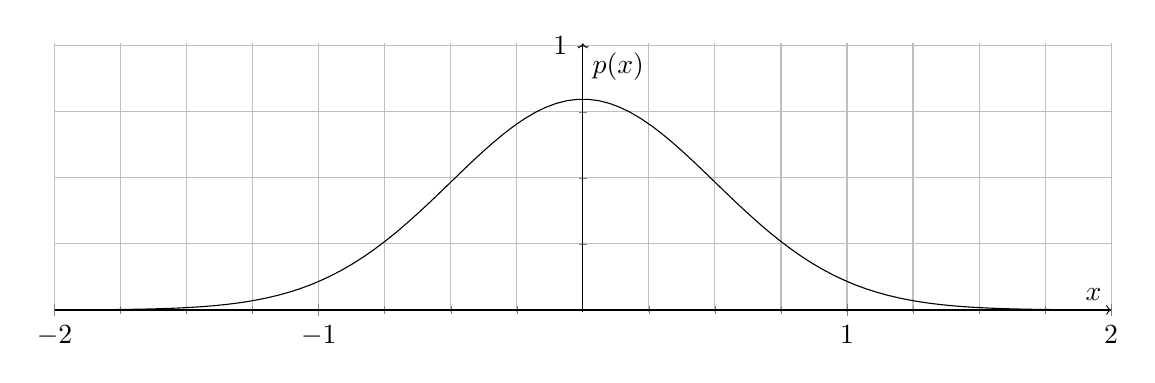
\begin{tikzpicture}
                \begin{axis}[
                    width = 15cm, height = 5cm,
                    trig format plots = rad,
                    grid = both,
                    xmin = -2,
                    xmax = 2,
                    ymin = 0,
                    ymax = 1,
                    axis equal,
                    axis x line = middle,
                    axis y line = middle,
                    axis line style = {->, color=black},
                    xtick distance = 1,
                    ytick distance = 1,
                    minor tick num = 3,
                    xlabel={$x$},
                    ylabel={$p(x)$},
                    ]
                    \addplot[domain=-2:2,samples=100]{1/sqrt(pi/2)*e^(-x^2*2)};
                \end{axis}
            \end{tikzpicture}
        \end{figure}\noindent
        $\operatorname{N}(0;1)$~--- стандартное нормальное распределение. Ещё оно обозначается $\Phi(x)$.
    \end{example}
    \begin{claim}
        Пусть $\xi=\operatorname{N}(\mu;\sigma^2)$, $\eta=a\xi+b$. Тогда
        $\eta=\operatorname{N}(a\mu_b;a^2\sigma^2)$.
    \end{claim}
    \begin{proof}
        Пусть $a>0$. Обозначим $y=ax+b$. Тогда
        \[\begin{split}
            P(\eta\leqslant t)&=P(a\xi+b\leqslant t)=P(\xi\leqslant\frac{t-b}a)=F_\xi(\frac{t-b}a)=\frac1{2\pi\sigma^2}\int\limits_{-\infty}^{\frac{t-b}a}\exp\left(-\frac{(x-\mu)^2}{2\sigma^2}\right)~\mathrm dx=\\
            &=\frac1{\sqrt{2\pi\sigma^2a^2}}\int\limits_{-\infty}^t\exp\left(-\frac{(\frac{y-b}a-\mu)^2}{2\sigma^2}\right)=\frac1{\sqrt{2\pi\sigma^2a^2}}\int\limits_{-\infty}^t\exp\left(-\frac{(y-b-a\mu)^2}{2a^2\sigma^2}\right)
        \end{split}\]
        Что и требовалось доказать. При $a<0$ аналогично.
    \end{proof}
    \begin{corollary}
        Если $\xi=\operatorname{N}(0;1)$, то $\sigma\xi+\mu=\operatorname{N}(\mu;\sigma^2)$.
    \end{corollary}
    \begin{example}
        Распределение Коши: $\operatorname{Cauchy}(x_0;\gamma)$.
        $$
        p(x)=\frac1{\pi\gamma}\cdot\frac1{1+\left(\frac{x-x_0}\gamma\right)^2}
        $$
        Тогда
        $$
        F(t)=\frac1{\pi\gamma}\int\limits_{-\infty}^t\frac{\mathrm dx}{1+\left(\frac{x-x_0}\gamma\right)^2}=\frac1\pi\atan\left(\frac{t-x_0}\gamma\right)+\frac12
        $$
    \end{example}
    \begin{example}
        Экспоненциальное распределение: $\operatorname{Exp}(\lambda)$.
        $$
        p(x)=\lambda e^{-\lambda x}\chi_{\mathbb R_+}
        $$
        Тогда
        $$
        F(t)=1-e^{-\lambda t}\chi_{\mathbb R_+}
        $$
    \end{example}
    \begin{example}
        $\Gamma$-распределение: $\Gamma(k,\lambda)$. Сначала для $k\in\mathbb N$, $\lambda>0$.
        $$
        p(x)=\frac{\lambda^kx^{k-1}}{(k-1)!}e^{-\lambda x}\qquad x\geqslant 0
        $$
        Для $k=\alpha>0$ заменим $(k-1)!$ на $\Gamma(\alpha)$.
    \end{example}
    \begin{claim}
        Пусть $\xi$~--- абсолютно непрерывная случайная величина с плотностью $p_\xi$. Пусть $g\in C^{(1)}(\mathbb R\to\mathbb R)$~--- строго монотонна. Пусть $\eta=g(\xi)$. Тогда
        $$
        p_\eta(y)=p_\xi(g^{-1}(y))\left|\frac{\mathrm d}{\mathrm dy}g^{-1}(y)\right|=p_\xi(g^{-1}(y))\left|\frac1{g'(g^{-1}(y))}\right|
        $$
    \end{claim}
    \begin{proof}
        Во-первых, у условиях теоремы $g^{-1}$ существует. Также второе равенство следует из первого в силу теоремы об обратном отображении.\\
        Не умаляя общности, $g$ строго возрастает. Тогда
        $$
        F_\eta(y)=P(g(\xi)\leqslant y)\overset{g\uparrow}=P(\xi\leqslant g^{-1}(y))=\int\limits_{-\infty}^{g^{-1}(y)}p_\xi(x)~\mathrm dx
        $$
        Продифференцировав это равенство по $y$ получим искомое равенство.
    \end{proof}
    \subparagraph{Сингулярные случайные величины и распределения.}
    \begin{definition}
        $x$ называется \textbf{точкой роста} монотонно возрастающей функции $f$, если $\forall\eps>0~f(x+\eps)-f(x-\eps)>0$.
    \end{definition}
    \begin{definition}
        Случайная величина $\xi$ (и её распределение) называются \textbf{сингулярными}, если $F_\xi\in C(\mathbb R)$ и мера множества точек $F_\xi$ роста равна нулю.
    \end{definition}
    \begin{example}
        Функция Кантора~--- функция, которая выглядит так: в нуле она равна нулю, в единице~--- единице, а во всех остальных точках строится так: отрезок $[0;1]$ делится на три части и в средней части равна среднему значению краёв (т.е. $\frac12$). И так далее.\\
        Оня является функцией распределения сингулярной случайной величины.
    \end{example}
    \begin{theorem}[Теорема Лебега]
        Пусть $F$~--- функция распределения. Тогда существуют единственные $F_{\mathrm{disc}}$, $F_{\mathrm{ac}}$ и $F_{\mathrm{sing}}$, которые в сумме дают $F$.\\
        Без доказательства.
    \end{theorem}
    \subsection{Многомерные случайные величины.}
    \paragraph{Распределение многомерных случайных величин.}
    \begin{definition}
        Вектор $\xi$ называется \textbf{случайным вектором} или \textbf{многомерной случайной величиной}, если $\xi_i$~--- случайная величина.
    \end{definition}
    \begin{definition}
        \textbf{Распределением случайного вектора} называется функция $P_\xi$, определённая на $\B^n$, заданная так:
        $$
        P_\xi(B_1;\ldots;B_n)=P(\{(\omega_1;\ldots;\omega_n)\mid\xi_1(\omega_1)\in B_1\land\cdots\land \xi_n(\omega_n)\in B_n\})
        $$
        Последнее обычно обозначается так: $P(\xi_1\in B_1,\xi_2\in B_2;\ldots;\xi_n\in B_n)$.
    \end{definition}
    \begin{definition}
        \textbf{Функцией распределения случайного вектора} $\xi$ называется функция
        $$
        F_\xi(t_1;\ldots;t_n)=P_\xi(\forall i\in[1:n]~\xi_i\leqslant t_i)
        $$
    \end{definition}
    \begin{claim}
        \[\begin{split}
            P(\forall i\in[1:n]~&a_i<\xi_i\leqslant b_i)=\\
            &F(b_1;b_2;\ldots;b_n)\\
            &-F(a_1;b_2;\ldots;b_n)-F(b_1;a_2;\ldots;b_n)-\cdots-F(b_1;b_2;\ldots;a_n)\\
            &+\vdots\\
            &\pm F(a_1;a_2;\ldots;a_n)
        \end{split}\]
        То есть в этой сумме участвует $F$ от $a_i$ и $b_i$ в произвольном сочетании, при этом минус стоит там, где нечётное количество $a_i$.
    \end{claim}
    \begin{proof}
        $$
            P(\forall i\in[1:n]~a_i<\xi_i\leqslant b_i)=P(\xi_1\leqslant b_1,\forall i\in[2:n]~a_i<\xi_i\leqslant b_i)-P(a_1\geqslant\xi_1,\forall i\in[2:n]~a_i<\xi_i\leqslant b_i)
        $$
        Проведя такую операцию несколько раз, получим искомое.
    \end{proof}
    \begin{remark}
        Если ввести обозначение $\Delta_{a_i;b_i}F=F(\cdot;\ldots;b_i;\cdot;\ldots;\cdots)-F(\cdot;\ldots;a_i;\cdot;\ldots;\cdots)$, то арифметическая сумма из утверждения выше записывается как
        $$
        \Delta_{a_1;b_1}\Delta_{a_2;b_2}\cdots\Delta_{a_n;b_n}F
        $$
    \end{remark}
    \begin{property}
        $$F(+\infty;\cdots;+\infty)=1$$
        $$F(-\infty;\cdots;-\infty)=0$$
        $F$ непрерывна справа.
    \end{property}
    \begin{theorem}
        Если функция распределения удовлетворяет трём свойствам выше, то она является функцией распределения некоторого случайного вектора.
    \end{theorem}
    \begin{proof}
        Аналогично одномерному случаю.
    \end{proof}
    \begin{definition}
        Случайный вектор (и его распределение) называется \textbf{дискретным}, если существует не более чем счётное множество $E$ такое что $P(\xi\in E)=1$.
    \end{definition}
    \begin{example}
        Полиномиальное распределение. Пусть $p=(p_1;\ldots;p_m)$, где $\sum p_i=1$. Обозначается $\operatorname{Poly}(n;p)$.\\
        Физическая интерпретация такая: мы бросаем кубик с $m$ гранями $n$ раз. Пусть $S_{n,j}$~--- количество исходов типа $j$ в $n$ независимых испытаниях. Тогда искомая случайная величина обладает распределением
        $$
        P(S_{n,1}\in B_1;S_{n,2}\in B_2;\ldots;S_{n,m}\in B_m)
        $$
        Рассмотрим $P(S_{n,1}=k_1;S_{n,2}=k_2;\ldots;S_{n,m}=k_m)$, где $\sum k_m=n$. Чему равна такая вероятность? Ну,
        $$
        \frac{n!}{k_1!k_2!\cdots k_m!}p_1^{k_1}p_2^{k_2}\cdots p_m^{k_m}
        $$
    \end{example}
    \begin{remark}
        Несложно заметить, что штука справа~--- слагаемые в сумме $(p_1+p_2+\cdots+p_m)^n$.
    \end{remark}
    \begin{definition}
        Случайный вектор $\xi$ (и его распределение) называется \textbf{абсолютно непрерывным}, если существует $p\in L(\mathbb R^n\to\mathbb R)$ с неотрицательными значениями такая что $P(\xi\in B)=\int_BP~\mathrm d\mu_n$ (тут интеграл $n$-кратный). В таком случае $p$ называется \textbf{плотностью} $\xi$.
    \end{definition}
    \begin{example}
        Случайный вектор $\xi$ имеет стандартное многомерное нормальное распределение $\operatorname{N}(\mathbb0_n;E_n)$, если его плотность равна
        $$
        p(x_1;\ldots;x_n)=\frac1{(\sqrt{2\pi})^n}\exp\left(-\frac{\sum\limits_{i=1}^nx_i^2}2\right)
        $$
    \end{example}
    \begin{property}
        Несложно заметить, что это произведение плотностей одномерных стандартных нормальных распределений.
    \end{property}
    \begin{example}
        Случайный вектор $\eta$ имеет многомерное нормальное распределение $\operatorname{N}(\mu;\Sigma)$ (где $\mu\in\mathbb R^n$, $\Sigma$~--- симметричная матрица $n\times n$ с неотрицательными собственными числами), если он равен $\sqrt\Sigma\xi+\mu$, где $\xi$~--- стандартный многомерный гауссовский вектор.
    \end{example}
    \begin{remark}
        В случае $\Sigma>0$ можно написать плотность:
        $$
        p(y)=\frac1{\sqrt{2\pi}^n\sqrt{\det\Sigma}}\exp\left(-\frac12(y-\mu)^T\Sigma^{-1}(y-\mu)\right)
        $$
    \end{remark}
 \end{document}
